% Contenuto di "143_capitoli/capitolo2/immagini_capitolo_2/confronto_vincoli_3d.tex"
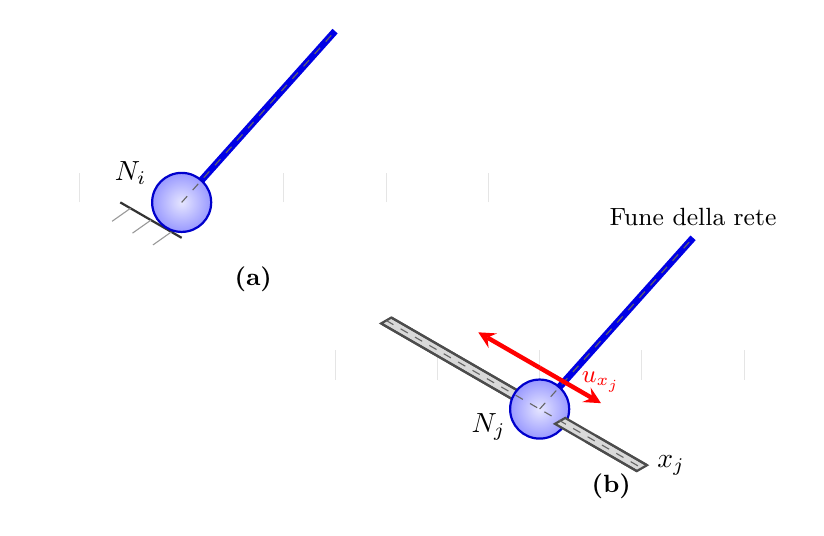
\begin{tikzpicture}[
    scale=1.5,
    x={(0.866cm,-0.5cm)}, y={(0.866cm,0.5cm)}, z={(0cm,1cm)},   % Assonometria isometrica
    guida/.style={draw=black!70, fill=gray!30, thick},
    fune/.style={draw=blue!90!black, line width=2.5pt},
    vettore/.style={->, >=stealth, red, ultra thick},
    titolo/.style={font=\small\bfseries, text=black, align=center}
]

    % =========================================================================
    % 1. SINISTRA: CERNIERA FISSA (Ancorata a terra)
    % =========================================================================
    
    % Piano di fondo locale
    \draw[gray!20, thin, step=0.5] (-1,-0.5,0) grid (1.5,1.5,0);
    
    % Piastra fissa di base a terra (Ancoraggio meccanico strutturale)
    \draw[black!80, thick] (-0.3,-0.3,0) -- (0.3,-0.3,0);
    \foreach \x in {-0.2,0,0.2} {
        \draw[black!40, thin] (\x,-0.3,0) -- (\x-0.08,-0.4,-0.1);
    }

    % Disegno della Fune (prima della sferetta per corretta sovrapposizione)
    \draw[fune] (0,0,0) -- (0.5, 1.0, 1.2);

    % Sferetta del nodo fisso (copre l'inizio della fune)
    \shadedraw[inner color=blue!10, outer color=blue!40, draw=blue!80!black, thick] (0,0,0) circle [radius=0.25cm];

    % Asse della fune (nero tratteggiato, sovrapposto sopra)
    \draw[dashed, black!60, thin] (0,0,0) -- (0.5, 1.0, 1.2);

    % Etichetta del nodo
    \node[black] at (-0.1, -0.4, 0.4) {$N_i$};
    
    % Titolo della subfigura a) bloccato alla quota y=0.5, z=-0.8
    \node[titolo] at (0.2, 0.5, -0.8) {(a)};


    % =========================================================================
    % 2. DESTRA: CERNIERA MOBILE (Su Guida Lineare)
    % =========================================================================
    % Lo shift ora è (3.5, 0, 0) puro: y=0 e z=0 sono identici al precedente.
    % Questo rende le due cerniere perfettamente parallele e complanari.
    \begin{scope}[shift={(3.5,0,0)}]
        
        % Piano di fondo locale
        \draw[gray!20, thin, step=0.5] (-1.5,-0.5,0) grid (1,1.5,0);

        % Guida cilindrica (asse x locale) - parte posteriore
        \fill[guida] (-1.5,-0.05,0) -- (0,-0.05,0) -- (0,0.05,0) -- (-1.5,0.05,0) -- cycle;
        \draw[black!70, thick] (-1.5,-0.05,0) -- (0,-0.05,0);
        \draw[black!70, thick] (-1.5,0.05,0) -- (0,0.05,0);

        % Disegno della Fune
        \draw[fune] (0,0,0) -- (0.5, 1.0, 1.2) node[above, black] {\small Fune della rete};

        % Sferetta del nodo mobile (copre l'inizio della fune e la parte posteriore della guida)
        \shadedraw[inner color=blue!10, outer color=blue!40, draw=blue!80!black, thick] (0,0,0) circle [radius=0.25cm];

        % Parte anteriore della guida
        \fill[guida] (0.2,-0.05,0) -- (1.0,-0.05,0) -- (1.0,0.05,0) -- (0.2,0.05,0) -- cycle;
        \draw[black!70, thick] (0.5,-0.05,0) -- (1.0,-0.05,0);
        \draw[black!70, thick] (0.5,0.05,0) -- (1.0,0.05,0) node[right, black] {$x_j$};
     
        % Asse geometrico della guida
        \draw[dashed, black!60, thin] (-1.5,0,0) -- (1.0,0,0);

        % Asse della fune (nero tratteggiato)
        \draw[dashed, black!60, thin] (0,0,0) -- (0.5, 1.0, 1.2);

        % Frecce dei Gradi di Libertà (Traslazione u_xj)
        \draw[vettore] (0,0,0.35) -- (0.6,0,0.35) node[above] {\small $u_{x_j}$};
        \draw[vettore] (0,0,0.35) -- (-0.6,0,0.35);

        % Etichetta del nodo
        \node[black] at (-0.1, -0.4, 0) {$N_j$};
        
        % Titolo della subfigura b) bloccato alla stessa identica coordinata relativa
        \node[titolo] at (0.2, 0.5, -0.8) {(b)};
        
    \end{scope}

\end{tikzpicture}